% $Id: msk-010.tex 9493 2021-10-26 22:07:41Z mskala $

%
% MSK 010 user/build manual
% Copyright (C) 2017, 2018, 2021  Matthew Skala
%
% This program is free software: you can redistribute it and/or modify
% it under the terms of the GNU General Public License as published by
% the Free Software Foundation, version 3.
%
% This program is distributed in the hope that it will be useful,
% but WITHOUT ANY WARRANTY; without even the implied warranty of
% MERCHANTABILITY or FITNESS FOR A PARTICULAR PURPOSE.  See the
% GNU General Public License for more details.
%
% You should have received a copy of the GNU General Public License
% along with this program.  If not, see <http://www.gnu.org/licenses/>.
%
% Matthew Skala
% https://northcoastsynthesis.com/
% mskala@northcoastsynthesis.com
%

\documentclass{ncmanual}

\title{MSK~010\quad Fixed Sine Bank}
\author{Matthew Skala}

\begin{document}

\maketitle

%%%%%%%%%%%%%%%%%%%%%%%%%%%%%%%%%%%%%%%%%%%%%%%%%%%%%%%%%%%%%%%%%%%%%%%%

\begin{copyrightpage}
Documentation for the MSK~010\\
Copyright \copyright\ 2017, 2018, 2021 Matthew Skala

\GPLThreeStatement
\end{copyrightpage}

\tableofcontents

%%%%%%%%%%%%%%%%%%%%%%%%%%%%%%%%%%%%%%%%%%%%%%%%%%%%%%%%%%%%%%%%%%%%%%%%

% $Id: general.tex 9828 2022-02-10 17:51:13Z mskala $

%
% MSK 014 general notes
% Copyright (C) 2022  Matthew Skala
%
% This program is free software: you can redistribute it and/or modify
% it under the terms of the GNU General Public License as published by
% the Free Software Foundation, version 3.
%
% This program is distributed in the hope that it will be useful,
% but WITHOUT ANY WARRANTY; without even the implied warranty of
% MERCHANTABILITY or FITNESS FOR A PARTICULAR PURPOSE.  See the
% GNU General Public License for more details.
%
% You should have received a copy of the GNU General Public License
% along with this program.  If not, see <http://www.gnu.org/licenses/>.
%
% Matthew Skala
% https://northcoastsynthesis.com/
% mskala@northcoastsynthesis.com
%

\chapter{General notes}

This manual documents the MSK~014 Gracious Host, which is a module for use
in a Eurorack modular synthesizer.  The module's main function is provide an
interface from USB devices, especially MIDI controllers, to the CV/gate
synthesizer.  As the name implies, the Gracious Host functions as an
embedded host, capable of connecting devices like keyboards without
needing the involvement of a separate computer.  It supports multiple
control modes for use in different kinds of patches, and the onboard
microcontroller can be reprogrammed in the field with new or modified
firmware loaded from a USB flash drive through the front-panel port.

This is one of two manuals.  The other manual is specifically intended for
programmers who are modifying or replacing the firmware, and is of less
interest for most users.

\section{Front panel connections}

The front panel of the Gracious Host is shown in
Figure~\ref{fig:panel-mockup}.  The fragment of music notation on the panel
spells GRACE as a pun on the module name:  treble clef (G clef); quarter-note
rest (R); and the three notes A, C, E.

\begin{figure*}
{\centering\setlength{\fboxsep}{0pt}\setlength{\fboxrule}{0.6pt}%
 \fbox{\includegraphics{panel-mockup.pdf}}\par}
\caption{Module front panel.}\label{fig:panel-mockup}
\end{figure*}

\subsection{Serial bus port}

The port at upper left is for connecting a USB device, such as a USB-MIDI
keyboard.  This is an \emph{embedded host} port, capable of supporting many
USB 1.0, 1.1, and 2.0 low-speed and full-speed devices relevant to
synthesizer use, but it does not support the entire USB standard with every
configuration of every device.  Exactly what the module will do depends on
what kind of device is plugged in; it will normally detect whenever a device
is inserted or removed, and go into a mode appropriate for that device, with
the different modes described in subsequent chapters of this manual.

The port is intended only for standard low-power devices such as MIDI
controllers.  The maximum current it is \emph{intended} to support is
100\,mA (which is a ``unit load'' according to the relevant USB
standards).  Some devices may attempt to draw more, and may succeed, but this
port is not intended for high-power applications like battery charging.

The Gracious Host cannot make use of a hub.  The USB device must be
attached directly to the port, and only one USB device can be attached at a
time.

\subsection{Control voltage inputs}

The top pair of jacks, labelled ``IN,'' serve as control voltage inputs,
which may be gate/trigger or pitch control voltages depending on the
operating mode.  Although the module will not be damaged by voltages between
the power supply rails ($\pm$12V when the module is powered up), the useful
range of voltages over which the analog-to-digital converters can work
properly is from 0V to $+$5V.

The nominal input impedance for these jacks is 100k$\Omega$.

\subsection{Bi-colour LEDs}

Immediately below the input jacks is a pair of bi-colour (red and green)
LEDs.  These display status information with a function that depends on the
operating mode.  For instance, in most MIDI-controller modes, the LED on one
side of the module will light when that side is playing a note.

\subsection{Control voltage (analog) outputs}

The second pair of jacks from the top, labelled ``CV,'' are multi-purpose
analog control voltage outputs with an intended operating range of 0V to
$+$5V.  These are typically used for things like pitch and velocity, again
depending on the mode.  In a few modes where these jacks are used for
trigger or gate output, they may produce a slightly higher uncalibrated
voltage like $+$5.5V.

\subsection{Gate (digital) outputs}

The bottom pair of jacks, labelled ``GT,'' produce digital control voltages
(gates or triggers), with ``low'' at 0V to within the tolerances of op amp
offsets, and ``high'' at approximately 9V.

\section{Specifications}

The nominal impedance for the input jacks is 100k$\Omega$.  All the outputs
are driven by op amps with in-the-loop 1k$\Omega$ resistors, giving them
effectively zero output impedance in normal use but limiting the output
current to about 10\,mA under short-circuit conditions.

Briefly shorting any input or output to any fixed voltage at or between the
power rails, or shorting two to each other, should be harmless to the
module.  Note that ``between the power rails'' does mean it is safer to feed
voltages into the module when power is applied, since without power, both
power rails will be at zero.  Patching the MSK~014's output into the output
of another module should be harmless to the MSK~014, but doing that is not
recommended because it is possible the other module may be harmed.

This module contains series reverse protection diodes and is unlikely to be
damaged by a reverse power connection, but because it uses a 16-pin power
connection, there are more kinds of misconnection possible than pure reversal
of the main power rails.  It is possible that there could be a short
circuit, more likely damaging to the power supply than to the module, if the
power is misconnected.  The connector on the module is polarized and
unlikely to be misconnected, but some caution is still recommended when
connecting the cable at the bus board.

The maximum current demand of this module in normal operation is 10\,mA from
the $+$12V supply, 20\,mA from the $-$12V supply, and a variable amount from
the $+$5V supply.  For power budgeting purposes I suggest counting the
Gracious Host's $+$5V requirement as 130\,mA, though the details are more
complicated, as described below.  Placing an unusually heavy load on the
outputs (for instance, with so-called passive modules, output-to-output
patching, or attempting to charge USB devices from the front-panel port) can
increase the power supply current beyond these levels.

In more detail:  the Gracious Host supplies $+$5V power more or less
directly from the Eurorack bus to the attached USB device, so the amount
drawn from the Eurorack bus will depend on what is attached to the
front-panel USB port.  The Gracious Host needs up to 30\,mA of $+$5V itself,
plus whatever is drawn by the USB device.  USB devices, according to the
relevant specifications, are supposed to draw at most 100\,mA and then
request more from the host if desired -- but the standard Gracious Host
firmware will never give the device permission to draw extra power.  Thus in
normal operation with standards-compliant devices, 130\,mA should be the
maximum consumption of $+$5V Eurorack power for the module and the attached
device.

Now, on the one hand, nearly all devices commonly expected to be used with
the Gracious Host will actually consume much less than 100\,mA; 5--20\,mA is
more typically expected, and so in actual practice the maximum total $+$5V
consumption is likely to be 35--50\,mA.  However, some high-power USB
devices actually draw more than the specified 100\,mA maximum without
following the protocol for requesting it.  The Gracious Host uses a PTC
thermistor, often called a thermal fuse although it really is not a fuse at
all, to protect against short circuits.  This protective device has a
\emph{hold current} of 200\,mA (meaning that at that level it will
not trip) and a \emph{trip current} of 400\,mA (meaning that at that level
it will trip in a few seconds).  So, if somewhat overloaded, the module
could consume as much as 230\,mA of Eurorack $+$5V power continuously; and
if heavily overloaded it could briefly draw much more before the thermal
fuse trips.

\section{Modification:  onboard $+$5V regulator}

\emph{The Gracious Host requires $+$5V power, up to 130\,mA under ordinary
recommended use.}

In the standard configuration, this module requires a power supply that
offers $+$5V.  It will not work if plugged into a stripped-down Eurorack
power supply with only $\pm$12V.  The decision was made to require
$+$5V because at present nearly all commercial Eurorack power supplies do in
fact offer $+$5V; the Gracious Host and the attached USB device each require
a significant amount of current, with the typically spiky demand of digital
circuitry; and attempting to convert $\pm$12V to $+$5V on board the module
would raise significant thermal, noise, and other technical issues, all just
to serve the small minority of users who have no $+$5V supply already.

However, for special purposes such as bench-top testing, it is possible to
solder in a 7805 regulator chip, on the pads next to the protection diodes,
as shown.  Photo depicts an early prototype with green solder mask instead
of production blue, and some minor differences in other details.  Then by
changing the configuration jumper settings (next section), the module can be
configured to draw its $+$5V current from the $+$12V instead, through the
installed regulator, with no requirement for an external $+$5V supply.

\nopagebreak\noindent
{\hspace*{\fill}\includegraphics[width=\linewidth]{optional-7805.jpg}\hspace*{\fill}\par} 

The 7805 regulator chip is not included in kits, and adding it is not a
recommended or supported configuration.  Depending on the amount of current
drawn by the external USB device, a 7805 installed as shown without a heat
sink may be liable to overheat.  Using an external device that needs maximum
rated power, or more, for more than a few seconds at a time may necessitate
adding a heat sink to the 7805 chip.  Furthermore, it is possible to set the
configuration jumpers in such a way that the on-board 7805 will be
cross-connected with the Eurorack bus -- meaning that it will attempt to
supply $+$5V power to other modules (possibly useful, but further increasing
the likelihood of overheating), or interfere with the existing bus $+$5V
supply if there is one after all.

The 7805, if installed, will have very little effect unless also activated
with the ``R'' jumper described below, so it remains possible to use a
modified module with bus power instead as long as you are careful with the
jumper configuration.

\section{Bus access and configuration jumpers}

There is a jumper block on the back of the module for selecting the $+$5V
source and whether to connect the first channel (left side of the front
panel) output jacks to the Eurorack bus.
\emph{At least one jumper (the one selecting $+$5V source) must be correctly
installed for the Gracious Host to operate at all.}

\nopagebreak\noindent
{\hspace*{\fill}\includegraphics[width=\linewidth]{jumpers.jpg}\hspace*{\fill}\par} 

Left to right, the jumper positions are:
\begin{itemize}
  \item ``G'':  install to connect left GT output to the ``gate'' bus;
  \item ``C'':  install to connect left CV output to the ``pitch CV'' bus;
  \item ``5'':  install to draw $+$5V power from the Eurorack bus;
  \item ``X'':  spare position, no effect; and
  \item ``R'':  install to draw $+$5V power from the onboard regulator, if
    one is installed -- otherwise no effect.
\end{itemize}

Four pins of the standard Eurorack bus are reserved for transmitting pitch
and gate CV among modules.  Most Eurorack cases will connect these pins
among modules -- usually with a separate CV/gate bus for each busboard in
multi-busboard systems.  Some of Doepfer's VCOs, like the A-110-1, receive
pitch CV from the bus by default when no pitch CV is connected to the front
panel, and North Coast's Middle Path VCO (the MSK~013) does the same. 
Modules like the Doepfer A-185-2 are capable of transmitting CV and gate
signals onto the bus.  Some Cwejman, Macbeth, MakeNoise, Malekko, MFB, Plan
B, Synthwerks, TipTop, and other manufacturers' modules also use these pins
in a compatible way.  So with compatible VCOs, you can just plug the
Gracious Host into the same busboard and have it control the VCO pitch
without needing to patch them with front-panel cables.  Similarly, you may
be able to have the gate signal from the Gracious Host activate envelopes or
VCAs without patching.

Some manufacturers have attempted to send digital signals over the CV/gate
bus in a non-standard way under the name ``sync bus.'' Despite more than one
using this name, each manufacturer attempting digital use of the bus has
defined its own nonstandard format for the signals (usually some variation
of MIDI adapted to voltage levels instead of current-loop), and they are not
in general compatible with each other.  Such use also is not compatible with
the analog use of the CV/gate bus as defined by Doepfer, and the two should
not be mixed.

To have the Gracious Host transmit pitch and gate CV onto the bus, install
jumpers in the first two positions, labelled ``G'' and ``C.'' These two
jumpers have the effect of connecting the output jacks directly to the bus. 
It is also possible to install just one of the two jumpers, to transmit only
pitch or only gate CV.  The standard or default configuration for assembled
modules sold by North Coast Synthesis is to install both these jumpers; but
it \emph{will} be necessary to remove them for good results if using more
than one Gracious Host on the same bus.  At most one module on a given
Eurorack bus should be configured to drive the CV/gate bus.  Setting up more
than one module as the bus master is equivalent to patching their outputs
into each other, and is unlikely to work well.

Install a jumper at the third position, labelled ``5,'' to connect the
Gracious Host's internal $+$5V supply to the Eurorack bus.  This should
always be done, for standard unmodified Gracious Host modules.  The only
reason not to install this jumper would be if the module has been modified
with an onboard regulator, in which case you could install the jumper in the
fifth position (``R'') instead, to use the installed onboard regulator.  It
would also be possible to install jumpers at both positions ``5'' and ``R,''
in which case the modified Gracious Host will attempt to regulate $+$12V
power down to $+$5V \emph{and also} supply that power to other modules
through the bus.  Doing so is potentially dangerous, but could possibly be
useful in a very small system where it might be desired to support some
other $+$5V module when the main power supply has no $+$5V rail.

The fourth jumper position (``X'') is unconnected, and the fifth (``R'')
is also unconnected in a standard build.  So, in an unmodified module, these
two jumper positions may be used as storage locations for the two extra
jumpers when CV/gate bus access is \emph{not} desired.  That way, there is
less risk of losing the jumpers.

\section{Source package}

A ZIP archive containing source code for this document and for the module
itself, including things like machine-readable CAD files, is available from 
the Web site at 
\url{https://northcoastsynthesis.com/}.  Be aware that actually building
from source requires some manual steps; Makefiles for GNU Make are provided,
but you may need to manually generate PDFs from the CAD files for inclusion
in the document, make Gerbers from the PCB design, manually edit the .csv
bill of materials files if you change the bill of materials, and so on.

Recommended software for use with the documentation and hardware source code
includes:
\begin{itemize}
  \item GNU Make;
  \item \LaTeX\ for document compilation;
  \item LaTeX.mk (Danjean and Legrand, not to be confused with other
    similarly-named \LaTeX-automation tools);
  \item Circuit\_macros (for in-document schematic diagrams);
  \item Kicad (electronic design automation);
  \item Qcad (2D drafting); and
  \item Perl (for the BOM-generating script).
\end{itemize}

The kicad-symbols/ subdirectory contains my customised schematic symbol and
PCB footprint libraries for Kicad.  Kicad doesn't normally keep dependencies
like symbols inside a project directory, so on my system, these files
actually live in a central directory shared by many projects.  As a result,
upon unpacking the ZIP file you may need to do some reconfiguration of the
library paths stored inside the project files, in order to allow the symbols
and footprints to be found.  Also, this directory will probably contain some
extra bonus symbols and footprints not actually used by this project,
because it's a copy of the directory shared with other projects.

The source package also contains source code for the module firmware, which
is written in PIC24 assembly language and documented in the \emph{MSK~014
Gracious Host Programmer's Manual}.  Working with that code will require
additional software tools -- in particular, Microchip's version of the GNU
assembly language toolchain.

The whole package is covered by the GNU GPL, version 3, a copy of which is
included in the file COPYING.

\section{PCBs and physical design}

The enclosed PCB design is for two boards, each
3.90$''$\linebreak[0]$\times$\linebreak[0]1.50$''$ or
99.06mm\linebreak[0]$\times$\linebreak[0]38.10mm.
The two boards are intended to
mount in a stack parallel to the Eurorack panel, held together with M3
machine screws and male-female hex standoff hardware.  See
Figure~\ref{fig:panel-stack}.  With 12mm of clearance for the power
connector and cable, the module should fit in about 39mm of depth measured from the
back of the front panel.

\begin{figure}
{\centering
\begin{tikzpicture}[scale=0.1]
  % power connector clearance
  \path[draw=black,dashed,thick] (27.2,-54.00) rectangle (39.2,-35.59);
  % panel
  \path[draw=black,fill=black!30!white] (-2.0,-64.25) rectangle (0,64.25);
  % panel-board 1 standoffs
  \path[draw=black,fill=white] (0,-32.93) rectangle (13,-26.93);
  \path[draw=black,fill=white] (0,51.72) rectangle (13,45.72);
  % board 1
  \path[draw=black,fill=blue!50!white] (13,-46.53) rectangle (14.6,52.53);
  % board 1-board 2 standoffs
  \path[draw=black,fill=white] (14.6,-32.93) rectangle (25.6,-26.93);
  \path[draw=black,fill=white] (14.6,51.72) rectangle (25.6,45.72);
  % board 2
  \path[draw=black,fill=blue!50!white] (25.6,-46.53) rectangle (27.2,52.53);
  % nuts and standoff thread ends at back
  \path[draw=black,fill=white] (27.2,-32.93) rectangle (29.2,-26.93);
  \path[draw=black,fill=white] (27.2,51.72) rectangle (29.2,45.72);
  \path[draw=black,fill=black!10!white] (29.2,-30.93) rectangle (31.2,-28.93);
  \path[draw=black,fill=black!10!white] (29.2,49.72) rectangle (31.2,47.72);
  % labels, arrows
  \node at (6.5,38) {\parbox{10mm}{\centering \small 13mm standoff}};
  \node at (20.1,38) {\parbox{11mm}{\centering \small 11mm standoff}};
  \node at (13,64) {\small 2mm front panel};
  \node at (21.4,60.5) {\small 2$\times$ 1.6mm PCBs};
  \draw[>=latex',->,very thick] (13.8,58.7) -- (13.8,53.0);
  \draw[>=latex',->,very thick] (26.4,58.7) -- (26.4,53.0);
  \node at (36.2,-18)
    {\parbox{17mm}{\centering \small 12mm clearance for mated power connector}};
  \draw (39.2,-55) -- (39.2,-64);
  \draw[>=latex',<->,thick] (0,-59.5) -- (39.2,-59.5);
  \node[fill=white] at (20.0,-59.5) {\small $\approx$39mm depth};
\end{tikzpicture}\par}
\caption{Assembled module, side view.}\label{fig:panel-stack}
\end{figure}

\section{Blink codes}

The two bi-colour LEDs on the front panel are used for multiple purposes. 
In most modes they light up in time with the notes being played.  They
flicker briefly when a USB device is inserted, both as a generic indicator
that something is happening, and to support debugging of the stages of the
USB attachment process.  But in some special situations the LEDs display
coded blinking patterns that report the module's status or error condition,
and these patterns are illustrated in this manual with diagrams like the
ones below.  Time reads left to right, with the entire diagram representing
a cycle that repeats every 1.05s.

If a hub is inserted in the USB port -- bearing in mind that the Gracious
Host does not work with hubs -- it will display bursts of four short red
flashes (Morse code ``H'' for ``hub'') on the right LED, leaving the left
LED dark, until the hub is removed.

\nopagebreak
\blinkcodeLR{}{}{}{0/0.5,1/1.5,2/2.5,3/3.5}

For an unsupported device other than a hub, the blink code is similar to the
one for ``hub,'' but the flashes are in a long-short-short pattern; Morse
code ``D'' for ``device unsupported.''

\nopagebreak
\blinkcodeLR{}{}{}{0/1.5,2/2.5,3/3.5}

In the event that something goes wrong inside a per-device USB driver and
the module is unable to recover while the device is attached, it displays
very fast back-and-forth red flashes until the device is removed.

\nopagebreak
\blinkcodeLR{}{0/0.5,1/1.5,2/2.5,3/3.5,4/4.5,5/5.5,6/6.5,7/7.5}%
{}{0.5/1,1.5/2,2.5/3,3.5/4,4.5/5,5.5/6,6.5/7,7.5/8}

If the module gracefully detects a trip of the USB polyfuse, indicating a
short circuit or that someone tried to charge a non-compliant high-power
device through the USB port, then in principle the firmware will try to
display a pattern of mostly red interrupted by short green flashes and
pauses.  Really, though, this display is unlikely to work; in actual testing
of an overloaded port condition the module is often sufficiently messed up
that it shuts off until power-cycled, or at least until the polyfuse cools
down.

\nopagebreak
\blinkcodeLR{3/3.5,5.5/6}{1/3,3.5/5.5,6/8}%
{1.5/2,7/7.5}{0/1.5,2/4,5/7,7.5/8}

There are other blink codes specific to the calibration procedure, which are
illustrated in the section on calibration.

\section{Use and contact information}

This module design is released under the GNU GPL, version 3, a copy of which
is in the source code package in the file named \texttt{COPYING}.  One
important consequence of the license is that if you distribute the design to
others -- for instance, as a built hardware device -- then you are obligated
to make the source code available to them at no additional charge, including
any modifications you may have made to the original design.  Source code for
a hardware device includes without limitation such things as the
machine-readable, human-editable CAD files for the circuit boards and
panels.  You also are not permitted to limit others' freedoms to
redistribute the design and make further modifications of their own.

I sell this and other modules, both as fully assembled products and
do-it-yourself kits, from my Web storefront at
\url{http://northcoastsynthesis.com/}.  Your support of my business is what
makes it possible for me to continue releasing module designs for free. 
The latest version of this document and the associated source files can be
found at that Web site.

Email should be sent to\\ \url{mskala@northcoastsynthesis.com}.

% $Id: warnings.tex 5678 2017-10-13 15:20:20Z mskala $

%
% MSK 010 safety and other warnings
% Copyright (C) 2017  Matthew Skala
%
% This program is free software: you can redistribute it and/or modify
% it under the terms of the GNU General Public License as published by
% the Free Software Foundation, version 3.
%
% This program is distributed in the hope that it will be useful,
% but WITHOUT ANY WARRANTY; without even the implied warranty of
% MERCHANTABILITY or FITNESS FOR A PARTICULAR PURPOSE.  See the
% GNU General Public License for more details.
%
% You should have received a copy of the GNU General Public License
% along with this program.  If not, see <http://www.gnu.org/licenses/>.
%
% Matthew Skala
% https://northcoastsynthesis.com/
% mskala@northcoastsynthesis.com
%

\chapter{Safety and other warnings}

Ask an adult to help you.

North Coast Synthesis Ltd.\ does not offer warranties or technical support
on anything we did not build and sell.  That applies both to modules built
by you or others from the kits we sell, and to fully-assembled modules that
might be built by others using our plans.  Especially note that because we
publish detailed plans and we permit third parties to build and sell modules
using our plans subject to the relevant license terms, it is reasonable to
expect that there will be modules on the new and used markets closely
resembling ours but not built and sold by us.  We may be able to help in
authenticating a module of unknown provenance; contact us if you have
questions of this nature.

For new modules purchased through a reseller, warranty and technical support
issues should be taken to the reseller \emph{first}.  Resellers buy modules
from North Coast at a significant discount, allowing them to resell the
modules at a profit, and part of the way they earn that is by taking
responsibility for supporting their own customers.

We also sell our products to hobbyists who enjoy tinkering with and
customizing electronic equipment.  Modules like ours, even if originally
built by us, may be quite likely to contain third-party ``mods,'' added or
deleted features, or otherwise differ from the standard specifications of
our assembled modules when new.  Be aware of this possibility when you buy a
used module.

Soldering irons are very hot.

Solder splashes and cut-off bits of component leads can fly a greater
distance and are harder to clean up than you might expect.  Spread out some
newspapers or similar to catch them, and wear eye protection.

Lead solder is toxic, as are some fluxes used with lead-free solder.  Do not
eat, drink, smoke, pick your nose, or engage in sexual activity while using
solder, and wash your hands when you are done using it.

Solder flux fumes are toxic, \emph{especially} from lead-free solder
because of its higher working temperature.  Use appropriate ventilation.

Some lead-free solder alloys produce joints that look ``cold''
(i.e.\ defective) even when they are correctly made.  This effect can be
especially distressing to those of us who learned soldering with lead solder
and then switched to lead-free.  Learn the behaviour of whatever alloy you  
are using, and then trust your skills.

Water-soluble solder flux must be washed off promptly (within less than an
hour of application) because if left in place it will corrode the metal. 
Solder with water-soluble flux should not be used with stranded wire because
it is nearly impossible to remove from between the strands.

Residue from traditional rosin-based solder flux can result in undesired
leakage currents that may affect high-impedance circuits, and this module
uses impedances into the megaohm range, where the leakage currents may have
some effect on circuit operation.  If your soldering leaves a lot of such
residue then it might be advisable to clean that off.

Voltage and current levels in some synthesizer circuits may be dangerous.

Building your own electronic equipment is seldom cheaper than buying
equivalent commercial products, due to commercial economies of scale from
which you as small-scale home builder cannot benefit.  If you think getting
into DIY construction is a way to save money, you will probably be
disappointed.

% $Id: bom.tex 9376 2021-08-31 13:12:43Z mskala $

%
% MSK 008 bill of materials
% Copyright (C) 2017  Matthew Skala
%
% This program is free software: you can redistribute it and/or modify
% it under the terms of the GNU General Public License as published by
% the Free Software Foundation, version 3.
%
% This program is distributed in the hope that it will be useful,
% but WITHOUT ANY WARRANTY; without even the implied warranty of
% MERCHANTABILITY or FITNESS FOR A PARTICULAR PURPOSE.  See the
% GNU General Public License for more details.
%
% You should have received a copy of the GNU General Public License
% along with this program.  If not, see <http://www.gnu.org/licenses/>.
%
% Matthew Skala
% https://northcoastsynthesis.com/
% mskala@northcoastsynthesis.com
%

\onecolumn
\chapter{Bill of materials}

{\centering
\fbox{This table is not a substitute for the text instructions.}

\begin{longtable}{rp{1.3in}cp{3in}}
  \textbf{Qty} & \textbf{Ref} & \textbf{Value/Part No.} & \\ \hline \endhead
\input{bomdata.tex}
\end{longtable}\par}

Not listed above, but also needed:  front panel, two circuit boards,
three 14-pin DIP sockets, solder, etc.
Fixed resistors should be 1\%\ metal film, except those specified as 0.1\%. 
North Coast Synthesis Ltd.\ kits or assembled modules sometimes contain
other parts with equivalent or better specifications rather than exact
manufacturers and part numbers shown here.

\twocolumn

% $Id: board2a.tex 9493 2021-10-26 22:07:41Z mskala $

%
% MSK 010 Board 2, variant A build instructions
% Copyright (C) 2017, 2018, 2021  Matthew Skala
%
% This program is free software: you can redistribute it and/or modify
% it under the terms of the GNU General Public License as published by
% the Free Software Foundation, version 3.
%
% This program is distributed in the hope that it will be useful,
% but WITHOUT ANY WARRANTY; without even the implied warranty of
% MERCHANTABILITY or FITNESS FOR A PARTICULAR PURPOSE.  See the
% GNU General Public License for more details.
%
% You should have received a copy of the GNU General Public License
% along with this program.  If not, see <http://www.gnu.org/licenses/>.
%
% Matthew Skala
% https://northcoastsynthesis.com/
% mskala@northcoastsynthesis.com
%

\chapter{Building Board 2 (Variant A)}

The recommended order for building this module is to assemble Board 2, the
one further from the front panel, first.  That will make it easier to get
all the physical positioning right for the components that bridge between
the boards or pass through the panel.  But before you start assembling Board
2, you must decide which variant you want to build.  Each one has a
different selection of eight nominal output frequencies.  Follow the
instructions in \emph{one} of the three ``Building Board 2'' chapters, depending on
which variant you want, before proceeding to the chapter called ``Building
Board 1.''  It's a choose your own module adventure!

\emph{This chapter contains the build instructions for Variant A, which has
the following nominal output frequencies and periods:}

\begin{tabular}{cc}
frequency & period \\ \hline
16mHz & 63s \\
60mHz & 16s \\
190mHz & 5.3s \\
410mHz & 2.4s \\
720mHz & 1.4s \\
1.3Hz & 750ms \\
4.8Hz & 210ms \\
16Hz & 63ms
\end{tabular}

If you have chosen Variant~A, use a permanent marker or some enamel paint to
fill in the ``A'' circle at the lower right of the front panel, so that you
can easily keep track of which module the one you're building now is, in a
system that might someday contain several MSK~010 modules.

Note that I'm describing a separate step for each component value,
and I built one that way in order to take a photo at each step, but if you
are reasonably confident about your skills you may find it easier to
populate all or most of the board (i.e.\ put the components in place) and
then solder them all at once.  Except where noted, the order in which you
add components does not matter much; but do note that you should solder the
board-to-board connector before the larger capacitors, because otherwise
they block access to it.

\section{Preliminaries}

Count out the right number of everything according to the bill of materials. 
There is an abbreviated BOM for Board~2, and a few items from Board~1 used
during the assembly of Board~2, in Table~\ref{tab:b2bom}.

\begin{table*}
{\centering
\fbox{This table is not a substitute for the text instructions.}
\vspace{\baselineskip}

\begin{tabular}{rp{1in}cp{3in}}
  \textbf{Qty} & \textbf{Ref} & \textbf{Value/Part No.} & \\ \hline
\input{bomdata-2a.tex}
\end{tabular}\par}
\caption{Bill of Materials for assembling Board~2.}\label{tab:b2bom}
\end{table*}

\section{Decoupling capacitors}

The four axial ceramic 0.1$\mu$F decoupling capacitors, C9, C10, C19, and
C20, are shown on the board by a special symbol without their reference
designators.

\noindent\includegraphics[width=\linewidth]{decoup-symbol.jpg}

Install these four capacitors where the symbol appears.  They are not
polarized and may be installed in either orientation.  These capacitors act
as filters for the power supplies to the op amp chips, reducing any coupling
of high-frequency noise between them and the rest of the synthesizer.

\noindent\includegraphics[width=\linewidth]{cap-decoup.jpg}

\section{Fixed resistors}

Resistors are never polarized.  I like to install mine in a consistent
direction for cosmetic reasons, but this is electrically unnecessary.  In
this module, metal film 1\%\ resistors are recommended for all fixed-value
resistors.  These will usually have blue bodies and four colour bands
designating the value, plus a fifth band (always brown\footnote{It also
happens, because of the way we choose resistor values, that the third band
will be black for all the resistors used in this module and nearly all the
resistors used in North Coast modules in general.}) for the tolerance,
and these are the types of resistors shipped in the North Coast kits.
Accordingly, I mention only the four value band colours for this type of
resistor; if you are using resistors with other codes, you are responsible
for knowing them.  Note that colour codes on metal film 1\% resistors are
often ambiguous (reading from one end or the other end may give two
different values, both plausible) and some of the colours are hard to
distinguish anyway.  If in doubt, always measure with an ohmmeter before
soldering the resistor in place.

The physical size of the resistors may vary, and details like the exact
colour of the bluish background.  You can see some of that variation in the
photos in these instructions.  Some of the resistance values used in this
module are hard to find, and we source different values from different
suppliers, so not all the resistors in a kit will necessarily be from the
same manufacturer, nor match on non-critical specifications like power
rating and physical size.

Install the eight 10k$\Omega$ (brown-black-black-red) resistors R1 to R4 and
R29 to R32.  These form part of the gain-control network for the amplifiers,
acting as a reference for the other components to balance against.  Do
not confuse these with similar-looking resistors for other power-of-ten
values, such as 1k$\Omega$ or 1M$\Omega$; those have the same colour code
except with the red replaced by other colours.

Be aware that one leg of each of these resistors is connected to the ground
plane of the circuit board, a fact evident from the cross-shaped pattern of
``thermal relief'' connections around the solder pad.  These joints, and
other grounded pins throughout the module, may require extra time and heat
to solder because each one is connected to large chunks of copper on both
sides of the board that tend to conduct heat away from the joint.  The
thermal relief design is supposed to reduce this effect, but in practice,
especially when using a low-wattage iron, it only helps to a limited degree.

\noindent\includegraphics[width=\linewidth]{res-10k.jpg}

Install the eight 22k$\Omega$ (red-red-black-red) resistors R9 to R12 and
R37 to R40.  These set the small-signal gain for the amplifiers by balancing
against the 10k$\Omega$ resistors.  Do not confuse these with the very
similar-looking 27k$\Omega$ resistors, which have the second band violet
instead of red.  Swapping the two values will result in bad output levels,
most likely too high with clipping, possibly too low.

\noindent\includegraphics[width=\linewidth]{res-22k.jpg}

Install the eight 27k$\Omega$ (red-violet-black-red) resistors R17 to R20
and R45 to R48.  These are coupled into the circuit under control of the
Zener diodes to reduce the gain as needed for the desired output levels.

\noindent\includegraphics[width=\linewidth]{res-27k.jpg}

The next eight resistor values (two of each) are installed in locations on
the board marked with reference designators (like ``R5'') but no values. 
That is because these are meant to be installed in different locations
depending on which variant of the module you are building.  The
correspondence between locations and values for Variant~A is shown in
Figure~\ref{fig:board-stuffing-2a}.  Follow the diagram and these
instructions carefully, because it is easy to make a mistake.

All these resistors are used to determine the frequencies of the
oscillators, two for each oscillator.  Installing the wrong timing resistor
value in one of the oscillators, but the same wrong value for both of the
two timing resistors, will result in oscillation at the wrong frequency. 
Installing two different resistor values in one oscillator will probably
result in its failure to oscillate at all.

\def\RVA{100k$\Omega$}\def\CVA{0.10$\mu$F}\def\TVA{63ms}\def\FVA{16Hz}
\def\RVB{150k$\Omega$}\def\CVB{0.22$\mu$F}\def\TVB{210ms}\def\FVB{4.8Hz}
\def\RVC{1.2M$\Omega$}\def\CVC{0.10$\mu$F}\def\TVC{750ms}\def\FVC{1.3Hz}
\def\RVD{1.0M$\Omega$}\def\CVD{0.22$\mu$F}\def\TVD{1.4s}\def\FVD{720mHz}
\def\RVE{390k$\Omega$}\def\CVE{1.0$\mu$F}\def\TVE{2.4s}\def\FVE{410mHz}
\def\RVF{1.8M$\Omega$}\def\CVF{0.47$\mu$F}\def\TVF{5.3s}\def\FVF{190mHz}
\def\RVG{5.6M$\Omega$}\def\CVG{0.47$\mu$F}\def\TVG{16s}\def\FVG{60mHz}
\def\RVH{10M$\Omega$}\def\CVH{1.0$\mu$F}\def\TVH{63s}\def\FVH{16mHz}

\begin{figure*}
\centering\begin{tikzpicture}
  \node at (0,0) {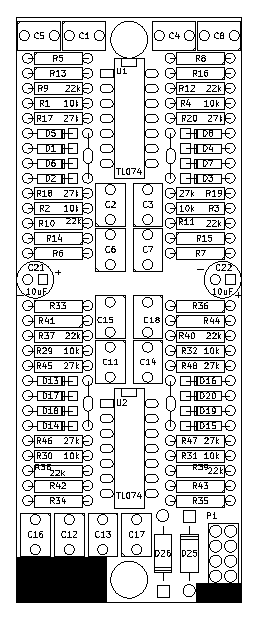
\includegraphics{rc2.eps}};
  \node[rectangle,draw,dashed,blue,very thick,inner sep=0.6cm]
    (o1) at (-1.15,4.4) {~~~~~~};
  \node[rectangle,draw,dashed,blue,very thick,inner sep=0.8cm]
    (o2) at (-1.0,1.4) {~~~~};
  \node[rectangle,draw,dashed,blue,very thick,inner sep=0.8cm]
    (o3) at (-1.0,-0.5) {~~~~};
  \node[rectangle,draw,dashed,blue,very thick,inner sep=0.65cm]
    (o4) at (-1.35,-3.53) {};
  \node[rectangle,draw,dashed,blue,very thick,inner sep=0.6cm]
    (o5) at (1.15,4.4) {~~~~~~};
  \node[rectangle,draw,dashed,blue,very thick,inner sep=0.8cm]
    (o6) at (1.0,1.4) {~~~~};
  \node[rectangle,draw,dashed,blue,very thick,inner sep=0.8cm]
    (o7) at (1.0,-0.5) {~~~~};
  \node[rectangle,draw,dashed,blue,very thick,inner sep=0.65cm]
    (o8) at (0.66,-3.53) {~~~~~~~~~~~~};
  \node at (-4.5,5.0) {\small\begin{tabular}{rl}
    \multicolumn{2}{c}{J5} \\
    C1, C5 & \CVA \\
    R5, R13 & \RVA \\
    $t$ & \TVA \\
    $f$ & \FVA
  \end{tabular}} edge[very thick,blue] (o1);
  \node at (-4.5,-0.7) {\small\begin{tabular}{rl}
    \multicolumn{2}{c}{J6} \\
    C11, C15 & \CVB \\
    R33, R41 & \RVB \\
    $t$ & \TVB \\
    $f$ & \FVB
  \end{tabular}} edge[very thick,blue] (o3);
  \node at (-4.5,1.8) {\small\begin{tabular}{rl}
    \multicolumn{2}{c}{J7} \\
    C2, C6 & \CVC \\
    R6, R14 & \RVC \\
    $t$ & \TVC \\
    $f$ & \FVC
  \end{tabular}} edge[very thick,blue] (o2);
  \node at (-4.5,-4.0) {\small\begin{tabular}{rl}
    \multicolumn{2}{c}{J8} \\
    C12, C16 & \CVD \\
    R34, R42 & \RVD \\
    $t$ & \TVD \\
    $f$ & \FVD
  \end{tabular}} edge[very thick,blue] (o4);
  \node at (4.5,-0.7) {\small\begin{tabular}{rl}
    \multicolumn{2}{c}{J1} \\
    C14, C18 & \CVE \\
    R36, R44 & \RVE \\
    $t$ & \TVE \\
    $f$ & \FVE
  \end{tabular}} edge[very thick,blue] (o7);
  \node at (4.5,1.8) {\small\begin{tabular}{rl}
    \multicolumn{2}{c}{J2} \\
    C3, C7 & \CVF \\
    R7, R15 & \RVF \\
    $t$ & \TVF \\
    $f$ & \FVF
  \end{tabular}} edge[very thick,blue] (o6);
  \node at (4.5,-4.0) {\small\begin{tabular}{rl}
    \multicolumn{2}{c}{J3} \\
    C13, C17 & \CVG \\
    R35, R43 & \RVG \\
    $t$ & \TVG \\
    $f$ & \FVG
  \end{tabular}} edge[very thick,blue] (o8);
  \node at (4.5,5.0) {\small\begin{tabular}{rl}
    \multicolumn{2}{c}{J4} \\
    C4, C8 & \CVH \\
    R8, R16 & \RVH \\
    $t$ & \TVH \\
    $f$ & \FVH
  \end{tabular}} edge[very thick,blue] (o5);
\end{tikzpicture}\par
\caption{Populating Board~2 for Variant~A}\label{fig:board-stuffing-2a}
\end{figure*}

Install the two 100k$\Omega$ (brown-black-black-orange) resistors R5
and R13.  Do not confuse these with other power-of-ten values.

\noindent\includegraphics[width=\linewidth]{res-100kA.jpg}

Install the two 150k$\Omega$ (brown-green-black-orange) resistors R33
and R41.

\noindent\includegraphics[width=\linewidth]{res-150kA.jpg}

Install the two 390k$\Omega$ (orange-white-black-orange) resistors R36
and R44.

\noindent\includegraphics[width=\linewidth]{res-390kA.jpg}

Install the two 1.0M$\Omega$ (brown-black-black-yellow) resistors R34
and R42.  Do not confuse these with other power-of-ten values.

\noindent\includegraphics[width=\linewidth]{res-1MA.jpg}

Install the two 1.2M$\Omega$ (brown-red-black-yellow) resistors R6 and
R14.

\noindent\includegraphics[width=\linewidth]{{res-1.2MA}.jpg}

Install the two 1.8M$\Omega$ (brown-gray-black-yellow) resistors R7
and R15.

\noindent\includegraphics[width=\linewidth]{{res-1.8MA}.jpg}

Install the two 5.6M$\Omega$ (green-blue-black-yellow) resistors R35
and R43.

\noindent\includegraphics[width=\linewidth]{{res-5.6MA}.jpg}

Install the two 10M$\Omega$ (brown-black-black-green) resistors R8 and
R16.  Do not confuse these with other power-of-ten values.

\noindent\includegraphics[width=\linewidth]{res-10MA.jpg}

\section{Board to board connectors}

It is important to solder the male header connector that links Board~2 to
Board~1 at this time, before adding the film and electrolytic capacitors,
because the capacitors surround the solder pads on the front of Board~2 in a
way that makes it difficult to work on the connector without damaging the
capacitors.  For best alignment, you should solder the male connector while
it is mated with the female connector on Board~1, and it's convenient to
solder the Board~1 connector at this time too.

Assemble the two boards and the two connectors using the M3 machine screws,
and 10mm and 11mm standoffs, as shown.  The 11mm standoffs should separate
the two boards; I suggest using the 10mm standoffs instead of hex nuts for
this temporary assembly because they're easier to tighten by hand.  Do not
confuse the two lengths.  Solder the connectors on both boards.  Then
disassemble them, and set aside the hardware and Board~1 for later.

\noindent\includegraphics[width=\linewidth]{b2b-stack.jpg}

\section{Semiconductors}

Install the sixteen 1N5229B 4.3V Zener diodes D1 to D8 and D13 to D20. 
These control the output level of the oscillators, by gradually bringing the
27k$\Omega$ resistors into the circuit as the level increases to back down
the gain until it reaches equilibrium.  They are polarized components and it
is important to install them right way round.  Each diode is packaged inside
a pink glass bead with a black stripe at one end; that end is the
\emph{cathode}.  The silkscreen markings on the board have a corresponding
stripe and the diodes should be installed with their stripes matching the
markings on the board.  The solder pads for the cathodes are also square
instead of round; and the diodes are arranged so that all the cathodes point
inward from the edge of the board.  Installing one of these diodes backwards
will probably result in the output level of the corresponding oscillator
being much too low, as well as some asymmetric (second harmonic) distortion
in the waveform.

\noindent\includegraphics[width=\linewidth]{zenerA.jpg}

The 1N5229B diodes are the only small glass diodes in an MSK~010 kit, but be
warned that if you're doing other electronic construction, then you will
probably have many other small glass diodes on hand (for instance, the very
popular 1N4148 general-purpose type) and they all look pretty much
identical, distinguished only by their electrical properties and
near-microscopic code numbers etched onto the glass.  Be careful not to mix
these diodes up with other types of diodes.  Substituting general-purpose
switching diodes in this circuit will probably give you output levels that
are much too high.

Install the two 1N5818 or SBA130 Schottky rectifier diodes D25 and D26. 
These are for reverse-voltage protection; they cut off power to the module
when the power plug is backwards.  They are polarized and it is important to
install them in the right direction.  As with the Zeners, these diodes will
be marked with stripes indicating their cathodes (here, probably white or
light grey paint on a black or dark grey plastic package) and those stripes
should match the stripes on the PCB silkscreen.  The cathode solder pads are
also square.  Installing these backwards means they will have the opposite
of the intended protective effect.

\noindent\includegraphics[width=\linewidth]{schottkyA.jpg}

Install the two 14-pin DIP sockets for the TL074 quad op amp chips, U1 and
U2.  These chips provide amplification to keep the oscillators running.  The
sockets themselves do not care which direction you install them, but it is
critically important that the chips installed in the sockets should be
installed in the right direction.  To help with that, the sockets will
probably be marked with notches at one end (indicating the end where Pin~1
and Pin~14 are located) and you should install the sockets so that the
notched ends match the notches shown on the PCB silkscreen.  The solder pad
for Pin~1 is also distinguished by being rectangular instead of rounded.

Installing DIP sockets without having them tilted at a funny angle can be
tricky.  I recommend inserting the socket in the board, taping it in place
on the component side with vinyl electrical tape, then soldering one pin on
one corner and checking that the socket is snug against the board before
soldering the other pins.  That way, if you accidentally solder the first
pin with the socket tilted, it will be easier to correct (only one pin to
desolder instead of all of them).

\noindent\includegraphics[width=\linewidth]{dip-2A.jpg}

If you somehow manage to solder an entire socket in backwards, don't try to
desolder it to turn it around.  Just leave it as it is and remember that
when you insert the chip, you must insert it so the chip matches the
markings on the \emph{board}, not the turned-around socket.

\section{Film capacitors}

The film capacitors in this module are used to determine oscillator timing. 
As with the timing resistors, they are marked on the PCB with their
references only, no capacitance values, because they are arranged
differently for the different module variants.  See
Figure~\ref{fig:board-stuffing-2a} for information on which capacitors go
where in this variant.

Be careful to identify the values of the capacitors correctly.  They may all
look very similar.  In some cases the physical sizes of the capacitors vary
with their value (for instance, 1.0$\mu$F will probably be bigger than
0.1$\mu$F), but there may also be different values the same physical size. 
Etched markings on the capacitors will probably use the symbol $\mu$ instead
of a decimal point, such as $\mu$1 to designate 0.1$\mu$F, as opposed to
1$\mu$ for 1.0$\mu$F.  Many digital multimeters will have a ``capacitor
test'' feature which you can use to confirm that you've identified the
capacitors correctly.  Installing the wrong capacitors in an oscillator
will give you the wrong frequency (in case of two capacitors that are the
same wrong value) or no oscillation (in case of two capacitors of different
values).

Also be careful about the physical aspects of installing the capacitors.  I
usually stick them in place with vinyl tape before soldering, but it's
difficult to get them to stay in at a nice angle.  If they're tilted over,
that is only really a cosmetic issue; the circuit should work fine as long
as both electrical connections are made.  These capacitors are also
unpolarized, and will work electrically regardless of the direction in which
they are installed.

Install the four 0.1$\mu$F film capacitors C1, C2, C5, and C6.

\noindent\includegraphics[width=\linewidth]{{cap-0.1uA}.jpg}

Install the four 0.22$\mu$F film capacitors C11, C12, C15, and C16.

\noindent\includegraphics[width=\linewidth]{{cap-0.22uA}.jpg}

Install the four 0.47$\mu$F film capacitors C3, C7, C13, and C17.

\noindent\includegraphics[width=\linewidth]{{cap-0.47uA}.jpg}

Install the four 1.0$\mu$F film capacitors C4, C8, C14, and
C18.\footnote{This photo shows the 10$\mu$F capacitors already installed, but
that's really the next step.}

\noindent\includegraphics[width=\linewidth]{{cap-1.0uA}.jpg}

\section{Electrolytic capacitors}

Install the two 10$\mu$F electrolytic capacitors C21 and C22, which filter
the power supply for the module as a whole.  These are polarized components
and they may explode if installed backwards.  Each one will be marked on its
casing with a stripe and minus signs to indicate the negative lead; the
positive lead will probably also be longer.  These clues should be matched
with the markings on the PCB: plus and minus symbols in the silkscreen and a
square solder pad for the positive (long) lead.

\noindent\includegraphics[width=\linewidth]{cap-10uA.jpg}

\section{Eurorack power connector}

Install the 2$\times$5-pin Eurorack power connector.  This connector is not
polarized in itself, although the connection it makes is polarized.  As with
the DIP sockets, you should be careful to get it installed snugly against
the board, not tilted at an angle.  Use vinyl tape or similar to hold it in
place, solder one pin, then check that it is straight before you solder the
other pins.

Be aware that both the connector and the copper connections to it on the PCB
have relatively large thermal mass.  These solder joints will need more
heat than usual; and after you have soldered it, the connector will remain
hot longer than recently-soldered components usually do.  Don't burn
yourself.

The six pins in the centre of the connector, that is all except the four
corner pins, are for grounding and they are all connected together on the
board.  Thus, if you accidentally form solder bridges among these six pins
while installing the connector, don't waste effort trying to remove them;
they will have no electrical effect.

\noindent\includegraphics[width=\linewidth]{powerA.jpg}

That's all the components for Board~2.

Because some connections on this board operate at multi-megaohm impedances,
it may be a good idea to clean the flux residue off of Board~2 even if you
are using no-clean flux which would not normally require cleaning.  For
this type of solder flux, or traditional rosin, use isopropyl alcohol for
cleaning.  If you used water-soluble solder flux, then cleaning is
mandatory and you should use water.

In between completed boards is a good time to take a break.

\input{board2b.tex}
\input{board2c.tex}
% $Id: board1.tex 9376 2021-08-31 13:12:43Z mskala $

%
% MSK 008 Board 1 build instructions
% Copyright (C) 2017, 2018  Matthew Skala
%
% This program is free software: you can redistribute it and/or modify
% it under the terms of the GNU General Public License as published by
% the Free Software Foundation, version 3.
%
% This program is distributed in the hope that it will be useful,
% but WITHOUT ANY WARRANTY; without even the implied warranty of
% MERCHANTABILITY or FITNESS FOR A PARTICULAR PURPOSE.  See the
% GNU General Public License for more details.
%
% You should have received a copy of the GNU General Public License
% along with this program.  If not, see <http://www.gnu.org/licenses/>.
%
% Matthew Skala
% https://northcoastsynthesis.com/
% mskala@northcoastsynthesis.com
%

\chapter{Building Board 1}\label{ch:board1}

Board~1 has components on both sides, and for best results, it is important
to install them in the right order.  Build Board~2 first, and see the
general comments in the Board~2 chapters about how to approach the task.

\section{Preliminaries}

Count out the right number of everything according to the bill of materials. 
There is an abbreviated BOM for the items needed in this chapter (including
the final assembly of the module) in Table~\ref{tab:b1bom}.  It
is also assumed you have a finished Board~2 from the previous chapter.

\noindent\includegraphics[width=\linewidth]{board1-parts.jpg}

\begin{table*}
{\centering
\fbox{This table is not a substitute for the text instructions.}
\vspace{\baselineskip}

\begin{tabular}{rp{1.3in}cp{3in}}
  \textbf{Qty} & \textbf{Ref} & \textbf{Value/Part No.} & \\ \hline
\input{bomdata-1.tex}
\end{tabular}\par}
\caption{Bill of Materials for Board~1.}\label{tab:b1bom}
\end{table*}

If you wish to reconfigure the CV2 inputs, you can change the solder jumpers
on Board~1 at this point.  In a standard build, the CV2 input on the left
channel \emph{adds} its voltage to CV1 and the quantizer output, while the
CV2 input on the right channel \emph{subtracts}.  This configuration is the
most useful one for most users and it is not particularly recommended to
change it.  But if you want to, first locate the jumpers on the board.  JP1
on the left is for the left channel and JP2 on the right is for the right
channel.

\noindent\includegraphics[width=\linewidth]{jumpers.jpg}

Each jumper has three terminals.  The middle one is connected to the one on
the left or the right for positive (adding) or negative (subtracting)
respectively, with a default set by a trace built into the circuit board. 
To change the jumper, use a sharp knife to carefully cut the connecting
trace, and then apply a blob of solder connecting the middle terminal to the
one for the opposite selection.  Use an ohmmeter to check that you have
really broken the connection on one side and recreated it on the other.

For a more advanced modification, you can solder fine wires into the holes
provided and run them into other circuitry of your own construction.  If you
add an SPDT switch, you could use it to change the add/subtract option by
flipping the switch.  You could also connect any number of additional
inverting and noninverting input jacks through 100k$\Omega$ precision
resistors (0.1\%\ or better) to the $+$ and $-$ terminals, which as shown on
the schematic diagram are op amp virtual ground summing nodes.

\section{Decoupling capacitors}

The two axial ceramic 0.1$\mu$F decoupling capacitors C7 and C8 are shown on
the board by a special symbol without their reference designators.

\noindent\includegraphics[width=\linewidth]{decoup-symbol.jpg}

\pagebreak

Install these two capacitors where the symbol appears.  They are not
polarized and may be installed in either orientation.  These capacitors act
as filters for the power supplies to the op amp chip, protecting them from
high-frequency crosstalk.

\noindent\includegraphics[width=\linewidth]{{cap-0.1u1}.jpg}

\section{Fixed resistors}

Resistors are never polarized.  I like to install mine in a consistent
direction for cosmetic reasons, but this is electrically unnecessary.  In
this module, most resistors are metal film 1\%\ type; a few are 0.1\%\
precision metal film resistors.  Both kinds will usually have blue bodies
and four colour bands designating the value, plus a fifth band for the
tolerance, and these are the resistors shipped in the North Coast
kits.  The tolerance band is brown for 1\%\ and violet for 0.1\%, but note
that we may occasionally ship better-tolerance resistors in the kits than
the specifications require, if we are able to source them at a good price.
Accordingly, I mention only the four value band colours for this type of
resistor; if you are using resistors with other codes, you are responsible
for knowing them.  Note that colour codes on metal film 1\% resistors are
often ambiguous (reading from one end or the other end may give two
different values, both plausible) and some of the colours are hard to
distinguish anyway.  If in doubt, always measure with an ohmmeter before
soldering the resistor in place.

There are no cases in this module of the same nominal resistance value being
used at more than one tolerance, but the 0.1\%\ resistance values are marked
with asterisks (*) on the board silkscreen as a reminder that these
positions require special resistors.

The physical size of the resistors may vary, and details like the exact
colour of the bluish background.  You can see some of that variation in the
photos in these instructions.  Some of the resistance values used in this
module are hard to find, and we source different values from different
suppliers, so not all the resistors in a kit will necessarily be from the
same manufacturer, nor match on non-critical specifications like power
rating and physical size.

Install the four 910$\Omega$ (white-brown-black-black) resistors R50, R52,
R53, and R54.  These form part of the current-controlling network for the
LED drivers.

\noindent\includegraphics[width=\linewidth]{res-910.jpg}

Install the two 1k$\Omega$ (brown-black-black-brown) resistors R47 and R48. 
These are current-limiting resistors to protect external circuits from
excessive output power on the module outputs; they also serve to isolate the
op amp chip from reactive (capacitive or inductive) loads that could make it
unstable.  Do not confuse these resistors with other power-of-ten values
such as 100k$\Omega$, which also have codes starting brown-black-black but
with different colours for the fourth, exponent-indicating, colour band.

\noindent\includegraphics[width=\linewidth]{res-1k.jpg}

Install the two 1.2k$\Omega$ (brown-red-black-brown) resistors R49 and R51. 
These form part of the current-controlling network for the LED drivers.

\noindent\includegraphics[width=\linewidth]{{res-1.2k}.jpg}

\pagebreak

Install the two 75k$\Omega$ (violet-green-black-red) resistors R13 and R16. 
These set the weight of the quantizer voltage inputs in comparison to the
manual octave switches.

\noindent\includegraphics[width=\linewidth]{res-75k.jpg}

Install the two 1M$\Omega$ (brown-black-black-yellow) resistors R15 and R16. 
These set the weight of the manual octave switches in the quantizers.  Do
not confuse them with other power-of-ten resistance values.

\noindent\includegraphics[width=\linewidth]{res-1M.jpg}

Install the ten 100k$\Omega$ 0.1\%\ precision resistors.  These control the
gain of the summing and inversion op amp circuits.  When building the
prototypes I noticed that either these resistors are just a little larger
than others of the same approximate body size, or maybe their leads are a
little stiffer; I found that I needed to bend the leads tighter (closer to
the bodies) than usual in order to have them fit nicely on the board.  Take
it slowly and carefully.

\noindent\includegraphics[width=\linewidth]{res-100k.jpg}

\section{Semiconductors}

Install the four 1N4148 or 1N914 switching diodes D14, D16, D18, and D20,
and D19.  These switch the LED drive currents.
They are polarized components and it is important to
install them right way round.  Each diode is packaged inside a pink glass
bead with a black stripe at one end; that end is the \emph{cathode}.  The
silkscreen markings on the board have a corresponding stripe and the diodes
should be installed with their stripes matching the markings on the board. 
The solder pads for the cathodes are also square instead of round. 
Installing one or more of these diodes backwards will result in incorrect
operation of the LEDs.

\noindent\includegraphics[width=\linewidth]{diodes1.jpg}

Install the 14-pin DIP socket for the TL074B quad low-offset operational
amplifier (op amp) U5.  This chip processes the CV1 and CV2 inputs,
inverting them as necessary, and does the final summation to drive the
module output.  The socket itself does not care which direction you install
it, but it is critically important that the chip installed in the socket
should be installed in the right direction.  To help with that, the socket
will probably be marked with a notch at one end (indicating the end where
Pin~1 and Pin~14 are located) and you should install the socket so that the
notched end matches the notch shown on the PCB silkscreen.  The solder pad
for Pin~1 is also distinguished by being rectangular instead of rounded.

Two of the holes for the capacitors C5 and C6 are located just off one end
of the DIP socket's footprint at the same spacing, making it possible to
insert the DIP socket shifted over one space with two of its pins in the
capacitor holes.  Be careful not to do that.

Installing DIP sockets without having them tilted at a funny angle can be
tricky.  I recommend inserting the socket in the board, taping it in place
on the component side with vinyl electrical tape, then soldering one pin on
one corner and checking that the socket is snug against the board before
soldering the other pins.  That way, if you accidentally solder the first
pin with the socket tilted, it will be easier to correct (only one pin to
desolder instead of all of them).

\noindent\includegraphics[width=\linewidth]{dip1.jpg}

\section{Compensation capacitors}

Install the two 33pF radial ceramic capacitors C5 and C6.  They will
probably be marked ``330,'' which means 33pF in a scheme similar to the
resistor colour code:  significant digits 3 3 to be followed by 0 zeroes. 
These capacitors help ensure stability of the op amp drivers by killing the
frequency response at ultrasonic frequencies, making parasitic oscillation
harder to sustain.

\noindent\includegraphics[width=\linewidth]{cap-33p.jpg}

\section{Panel components}

Fasten the 10mm and 11mm standoffs to Board~1.  The 11mm standoffs
should be on the same side of the board as the resistors and other
components, with their male ends sticking up as shown; they will separate
the two boards when the module is fully assembled.  The 10mm standoffs
should be on the other side, where they will separate the circuit boards
from the panel, with their male ends through the holes in the board to mate
with the 11mm standoffs.  \emph{Do not confuse the two similar lengths of
standoffs.}  Arranging them wrong at this stage may result in soldering panel
components at the wrong spacing in a way that will eventually make it
impossible to assemble the module correctly.
There is an exploded diagram for the final module on
page~\pageref{fig:exploded}.  You may wish to consult it if the way the
hardware fits together is at all unclear.

\noindent\includegraphics[width=\linewidth]{standoffs.jpg}

\pagebreak

Place (do not solder yet) the LEDs D11 and D12 in their corresponding holes
on the board.  Single LEDs are polarized and can be destroyed by reverse
voltage.  These ones here are special bi-colour devices with two separate
LEDs in each package.  The internal connection is such that each one
protects the other from reverse voltage; so if connected backwards, they
will not be destroyed, but the intended green and red colours will be
swapped.  Each LED lens has one flat side, and one leg shorter than the
other on that side.  The short leg is Pin~1.  Its proper place on the board
is marked by a circle with a flattened side matching the direction of the
flattened side on the LED lens, and an oval solder pad.  The other leg
(Pin~2, long, farther from the flat side) goes into the rectangular solder
pad.  Be sure both LEDs are placed right way around according to these
clues.

\noindent\includegraphics[width=\linewidth]{led.jpg}

Place (do not solder yet) the eight jack sockets J1 to J8 in their
corresponding holes on the board.  Their arrangement of legs and
corresponding slotted holes is such that they will only fit one way.

\noindent\includegraphics[width=\linewidth]{sockets.jpg}

Place (do not solder yet) the two toggle switches SW1 and SW2 in their
corresponding holes on the board.  The electrical connections on these
switches are symmetrical, but there is a keyway or groove on the threaded
bushing of each switch, and the keyway must be oriented downward for the
mounting hardware to fit properly later.

\noindent\includegraphics[width=\linewidth]{keyways.jpg}

Put the panel in place over the board so that the jack socket and toggle
switch bushings go through the corresponding holes in the panel and the
standoff line up behind their corresponding holes.  It may require some
careful adjustment of the jack socket locations to get them all through the
panel properly.  Check that the keyways on the toggle switch bushings are
facing downward, towards the small panel holes that will accept the tabs
from the locking rings.  Attach the panel firmly with the machine screws.

Use the knurled nuts that came with the jacks, to attach those to the panel. 
Beware of damaging the panel with wrenches, pliers, and similar.  If you
must use pliers, wrap them with tape to reduce the risk of scratches; but
just screwing the nuts on with finger pressure should be sufficient.

Use the hardware that came with the switches to attach them to the panel. 
In order starting closest to the panel, there should be a locking ring with
a tab that fits into the keyway on the switch bushing and another tab that
fits into the small hole on the panel; a toothed lockwasher; and at least
one hex nut.\footnote{These switches usually come with two nuts, but one is
probably sufficient given the use of the toothed lockwasher.} If the locking
ring will not fit because you mounted the switch backwards with the keyway
on the opposite side, this is your last chance to fix it.

Turn the assembly over so that the LEDs fall into place.  Adjust them by
gently pulling or pushing their legs until they all pass through the panel
holes by whatever amount you prefer.  If they are very loose, it may be
necessary to use sticky tape to temporarily hold them at the right depth,
but such a measure is unlikely to be needed; the holes are designed to be a
moderately snug friction fit on the LED lenses.

Solder all the jack sockets, LEDs, and switches.  The jack sockets and
switches may require a relatively large amount of solder to fill the
corresponding holes, but these joints are structural and should not be
neglected.  The LEDs, on the other hand, are sensitive to soldering heat and
should not be given excessive amounts of solder and heating, though the
joints must at least be strong enough not to break if users should
accidentally press on the LED lenses.

\section{Final assembly}

Insert the TL074B chip in its socket on Board~1.  Be careful to insert it
right way round:  the end with Pin 1 will be marked by an
indentation at one corner or a notch in the end and this end of the chip
should be inserted to match the notch in the socket and on the board
silkscreen and the rectangular Pin 1 solder pad.  The Pin 1 end of the chip
is at the bottom when the module is inserted in a rack.

Also be careful that all the legs of the chip go into the corresponding
holes in the socket.  These chips, when brand new, usually have their legs
splayed outward a little bit (a measure intended to help them fit snugly
into circuit boards when used without a socket) and you must gently bend the
legs inward in order to fit them in the sockets.  If you apply
pressure to a chip prematurely, without all the legs properly fitting into
the holes, it is easy to have the legs fold up or even break off.

It should not be necessary to remove the panel from Board~1 again.  Just
attach Board~2, carefully fitting its header
plug into the header socket on Board~1 and the male ends of the spacers
through the corresponding holes in Board~2.  Then use the hex nuts to fasten
Board~2 in place.

Insert the two LM339 chips in their sockets on Board~2.  Be careful to
insert them right way round, with the Pin~1 marking on the chip matching
those on the board, pointing downward when the module is inserted in a rack. 
As with the TL074B, be careful all the legs are in the holes of the socket
before you press the chip down, lest you fold up the delicate legs.

There is a rectangular white area at the lower left corner of Board~2
reserved for adding a serial number, signature, quality control marking, or
similar.  Use a fine-tipped permanent marker to write whatever you want
there.  Isopropyl alcohol will probably dissolve marker ink, so do this step
after any board-cleaning.

Your module is complete.

\noindent\includegraphics[width=\linewidth]{finished.jpg}

% $Id: testing.tex 5679 2017-10-13 15:24:08Z mskala $

%
% MSK 008 testing and adjustment instructions
% Copyright (C) 2017  Matthew Skala
%
% This program is free software: you can redistribute it and/or modify
% it under the terms of the GNU General Public License as published by
% the Free Software Foundation, version 3.
%
% This program is distributed in the hope that it will be useful,
% but WITHOUT ANY WARRANTY; without even the implied warranty of
% MERCHANTABILITY or FITNESS FOR A PARTICULAR PURPOSE.  See the
% GNU General Public License for more details.
%
% You should have received a copy of the GNU General Public License
% along with this program.  If not, see <http://www.gnu.org/licenses/>.
%
% Matthew Skala
% https://northcoastsynthesis.com/
% mskala@northcoastsynthesis.com
%
\chapter{Adjustment and testing}

The MSK~008 is designed to produce accurate output voltages, a goal partly
achieved through the use of precision components and partly by adjusting
trimmers to compensate for any remaining inaccuracies.  To perform the
adjustment steps you will need an accurate voltage standard (usually, a
good-quality multimeter) to compare against, and at least one patch cable.

For general troubleshooting and testing, you will also need a suitable power
supply and a multimeter.  An oscilloscope is not required, though optional
testing steps using one will be described.

\section{Short-circuit test}

With no power applied to the module, check for short circuits between the
three power connections on the Board~2 Eurorack power connector.  The two
pins at the bottom, marked with white on the circuit board, are for -12V. 
The two at the other end are for +12V; and the remaining six pins in the
middle are all ground pins.  Check between each pairing of these three
voltages, in both directions (six tests in all).  Ideally, you should use a
multimeter's ``diode test'' range for this; if yours has no such range, use
a low resistance-measuring setting. It should read infinite in the reverse
direction (positive lead to $-$12V and negative lead to each of the other
two, as well as positive lead to ground and negative to $+$12V) and greater
than 1V or 1k$\Omega$ in the forward direction (reverse those three
tests).  If any of these six measurements is less than 1k$\Omega$ or 1V,
then something is wrong with the build, most likely a blob of solder
shorting between two connections, and you should troubleshoot that before
applying power.

\emph{Optional}:  Although we test all cables before we sell them, bad
cables have been known to exist, so it might be worth plugging the Eurorack
power cable into the module and repeating these continuity tests across the
cable's corresponding contacts (using bits of narrow-guage wire to get into
the contacts on the cable if necessary) to make sure there are no shorts in
the cable crimping.  Doing this \emph{with the cable connected to the
module} makes it easier to avoid mistakes, because the module itself will
short together all wires that carry equal potential, making it easier to be
sure of testing the relevant adjacent-wire pairs in the cable.

Plug the module into a Eurorack power supply and make sure
neither it nor the power supply emits smoke, overheats, makes any unusual
noises, or smells bad.  If any of those things happen, turn off the power
immediately, and troubleshoot the problem before proceeding.

\emph{Optional}: Plug the module into a Eurorack power supply
\emph{backwards}, see that nothing bad happens, and congratulate yourself on
having assembled the reverse-connection protective circuit properly. 
Reconnect it right way round before proceeding to the next step.

\section{Blinking lights}

Plug the module into a Eurorack power supply, look at the lights on the
front, and flip the switches.  With a channel's switch down ($-$1 position)
the light for that channel should be green; with it up ($+$1 position), the
light should be red; and with it in the middle (0), the light should be
unilluminated.

\section{Output voltage adjustment}

Identify the three trimmers on the back of the module (Board~2).  The basic
concept here is that each channel has five output voltages from $-$2V to
$+$2V.  There is a trimmer (R27 for the left channel and R32 for the right)
which controls the level of the $-$2V output voltage separately per channel. 
Then there is also a third trimmer (R3) which adjusts the spacing between
the steps, for both channels; as a result its effect is greatest on the
$+$2V levels.  Nonetheless we will do the finest adjustments on these
trimmers by examining the $-$1V and $+$1V levels, because those are easier
to generate and test (given that $\pm$2V is full scale on many multimeters)
and choosing points nearer the middle helps distribute residual errors.

\noindent\includegraphics[width=\linewidth]{trimmer-ids.jpg}

For this adjustment procedure you will need to apply power to the module,
and check the output voltages on the two channels under different switch
settings.  If you have a spare 3.5mm jack socket it may be convenient to
make a little adapter for testing the voltage on an output jack using the
socket, a patch cable, and clip-on multimeter probes.  Otherwise, you can
just press the probes against the bare end of a patch cable, or use
alligator clips or similar.  Attempting to probe into the back of Board~1
with pointed probes will probably work, but may be annoying and fiddly.

\textit{Step 1:}  First you will adjust R27 on the $-$2V output of the left
channel.  Patch the output of
the right channel into the quantizer input of the left channel, and switch
both toggle switches to the $-$1 position (both LEDs should glow green). 
Measure the output voltage of the left channel and adjust R27 to bring it
close to $-$2V.  Perfection is not necessary here.  You will be adjusting it
again later; but getting it nearly right at this stage will make the later
adjustments, which interact, much easier.

\noindent\includegraphics[width=\linewidth]{test-patch.jpg}

\textit{Step 2:}  Switch both toggle switches to the $+$1 position (both
LEDs should glow red).  Measure the output voltage of the left channel and
adjust R3 to bring it close to $+$2V.

\textit{Step 3:}  Reverse the patch:  output of left channel into QUA input
of right channel, voltmeter to measure output of right channel.  Switch both
toggle switches to $-$1, and adjust R32 to bring it close to $-$2V. 
\emph{Then remove the patch cable between the two channels.}

\textit{Step 4:}  Measure the output of the left channel.  Switch its toggle
switch to $-$1, and adjust R27 to bring its output as close to $-$1.000V as
possible.

\textit{Step 5:}  Switch the left channel toggle switch to $+$1, and adjust
R3 to bring its output voltage as close to $+$1.000V as possible.

\textit{Step 6:}  Connect the voltmeter to the right channel.  Set the right
channel's toggle switch to $-$1, and adjust R32 to bring its output voltage
as close to $-$1.000V as possible.

\textit{Step 7:}  Repeat steps 4, 5, and 6 a second time.

Completing these steps as described should be enough to get all the quantizer
output voltages as accurate as the components and your test equipment allow.
Without guarantee, this will normally be better than $\pm$1mV on
all the output voltages.  If you have a lot of patience, you can attempt to
split any remaining error on R3 between the two channels.

If it seems necessary to turn a trimmer all the way to the end of its range,
and especially if even doing so does not allow you to hit the desired output
voltages, then something is wrong; see the troubleshooting suggestions next
section.

\section{Troubleshooting}

It would require several books to convey all the skills and knowledge useful
in troubleshooting even a simple electronic circuit like this one, but here
are some possible symptoms and some suggestions on diagnosis and treatment.

No response from the module at all; \emph{none} of the lights light up, no
signal on the output.  Most likely a power problem, such as a power cable
plugged in wrong or a short circuit.  It might even be a problem in the
power supply and not the module itself.

Module responds, but not as expected:  first attempt to localize the
problem.  Do signals on the CV1 and CV2 inputs appear correctly at the
output (though possibly with DC shifts, and with inversion on inverting CV2
signals)?  If not, check the summing circuits (U5 and associated components)
on Board~1 for problems.  Do voltages on the QUA inputs result in the
expected quantized voltages on the outputs?  If not, look at the quantizers
on Board~2, involving U3 and U4.  Note U3 detects the positive switching
thresholds for both channels and U4 detects the negative thresholds for both
channels; it is not one channel per chip.

If the quantizer appears to operate at all, but input thresholds or output
voltages seem to be wrong: check the voltages along the R8--R12 string for
the nominal values shown on the schematic, though these may correctly
\emph{not} have exactly the values shown if the adjustment procedure has
modified them to compensate for inaccuracies elsewhere.  They should at
least be close.  Wildly incorrect voltages along this string may indicate
problems with the voltage generator section (see circuit explanation),
including U1, U2, and the components near them on Board~2.  Check for solder
bridges on U1 and U2, with an ohmmeter as well as visually.

If the voltages along the resistor string are correct but the quantizer
output or LED responses are wrong, especially if the chips or LED-associated
components get noticeably hot: check for reversed switching diodes.

General tips for debugging DIP ICs:  make sure for, for each IC, that
\begin{itemize}
  \item it really is the type of IC it's supposed to be, not something else
    (beware of cheap ICs you buy from Chinese sellers on eBay, though the
    ones in this project are common enough in more reputable channels that
    you probably wouldn't have attempted that anyway);
  \item it is plugged in snugly;
  \item all the legs of the chip go nicely into the corresponding holes in
    the socket, with none bent outside or folded up under the chip;
  \item it is plugged in \emph{at all} (forgetting to do so is a surprisingly
    common mistake!);
  \item it is plugged in the right way around, with the Pin 1
    indentation or notch at the top and matching the other clues on the
    board (if this is wrong, the chip is probably destroyed and will need to
    be replaced);
  \item there are no solder bridges on the chip socket, unsoldered pins,
    debris clogging the socket holes, or similar;
  \item its decoupling capacitors (the small ceramic ones) are installed and
    there is nothing wrong with their solder joints; and
  \item in the case of the two LM339 chips, try swapping them and see if that
    makes any difference.
\end{itemize}

% $Id: patches.tex 5703 2017-10-31 03:07:37Z mskala $

%
% MSK 007 patch ideas
% Copyright (C) 2017  Matthew Skala
%
% This program is free software: you can redistribute it and/or modify
% it under the terms of the GNU General Public License as published by
% the Free Software Foundation, version 3.
%
% This program is distributed in the hope that it will be useful,
% but WITHOUT ANY WARRANTY; without even the implied warranty of
% MERCHANTABILITY or FITNESS FOR A PARTICULAR PURPOSE.  See the
% GNU General Public License for more details.
%
% You should have received a copy of the GNU General Public License
% along with this program.  If not, see <http://www.gnu.org/licenses/>.
%
% Matthew Skala
% https://northcoastsynthesis.com/
% mskala@northcoastsynthesis.com
%

\chapter{Patch ideas}

Here's a basic subtractive synthesis patch:  pitch CV from the MIDI
interface connects to the V/octave inputs on a sawtooth oscillator and the
MSK~007, while the gate CV drives and ADSR envelope which controls the
built-in VCA on the MSK~007 (VCA mode switch set to ``output'').

\nopagebreak\noindent
{\hspace*{\fill}\includegraphics[scale=0.6]{patch1.png}\hspace*{\fill}\par} 

In a more elaborate subtractive synthesis patch, two ADSR envelopes drive
the amplitude and filter cutoff separately, with an external VCA which frees
the MSK~007's built-in VCA to provide feedback.

\nopagebreak\noindent
{\hspace*{\fill}\includegraphics[scale=0.45]{patch2.png}\hspace*{\fill}\par} 

Deluxe subtractive synthesis patch demonstrating the use of the MSK~007 with
other North Coast Synthesis modules: the pitch CV goes through an MSK~008
Octave Switch (normalled to both channels) to provide separate manual octave
switching up and down for the VCO and the filter.  A sine wave from the
MSK~010 controls linear frequency modulation of the filter cutoff for a
unique effect.

\nopagebreak\noindent
{\hspace*{\fill}\includegraphics[scale=0.45]{patch3.png}\hspace*{\fill}\par} 

\pagebreak

The MSK~007 can be a minimal synth voice all by itself, using the
gate input to control the VCA in feedback mode to switch oscillation on and
off.  A MIDI interface is shown, but any CV-gate controller would work.

\nopagebreak\noindent
{\hspace*{\fill}\includegraphics[scale=0.6]{patch4.png}\hspace*{\fill}\par} 

An envelope generator set up to create a spike (fast attack and decay,
zero sustain level) can ``ping'' the filter when fed into the audio input. 
Set the VCA to feedback mode and adjust the level to the point where it
almost, but not quite, sustains oscillation.

\nopagebreak\noindent
{\hspace*{\fill}\includegraphics[scale=0.6]{patch5.png}\hspace*{\fill}\par}

Pinging with a noise burst instead of just a voltage spike produces a
different sound with some extra grit in the attack.

\nopagebreak\noindent
{\hspace*{\fill}\includegraphics[scale=0.6]{patch6.png}\hspace*{\fill}\par} 

\pagebreak

The MSK~007 can take inputs all the way down to DC, so
with the cutoff frequency very low (at or near its minimum) it can process
control voltages as
an unusual kind of slew rate limiter, with a bit of bounce or overshoot on
rapidly-changing inputs (especially in feedback mode).  The gain through the
filter is not easy to adjust to precisely unity, so you might not want to
use this for critical melodic material; but with a square wave LFO input, as
shown, it puts an interesting twist on the control waveform for generating
a drone texture.

\nopagebreak\noindent
{\hspace*{\fill}\includegraphics[scale=0.6]{patch7.png}\hspace*{\fill}\par} 

Doepfer's A-188-1 bucket brigade module does not include an output filter,
so at low clock rates the clock will be audible unless you filter it out
externally.  The MSK~007 is especially well-suited for that because of its
low cutoff.  With the MSK~007 tuned to cut off at the Nyquist frequency
(half the BBD's clock frequency), it will cleanly eliminate both clock and
alias signals.

\nopagebreak\noindent
{\hspace*{\fill}\includegraphics[scale=0.6]{patch8.png}\hspace*{\fill}\par} 

Spectral inversion is another use for a sharp low-pass filter.  Tune the
sine wave VCO (here used as a \emph{local oscillator}) to generate a carrier
a little above the highest frequency in the input.  Ring-modulate
(four-quadrant multiply) the input with the carrier.  That produces two
frequency bands: upper sideband consisting of the input shifted up by the
carrier frequency, and lower sideband consisting of all the input
frequencies subtracted from the carrier frequency.  The MSK~007
removes the upper sideband and any carrier feedthrough.

Spectral inversion is an interesting effect in itself, but you can also use
two copies of this patch (two MSK~007 modules, two oscillators,
and two channels of four-quadrant multiplication) with slightly
different carrier frequencies, to serve as a frequency shifter.

\nopagebreak\noindent
{\hspace*{\fill}\includegraphics[scale=0.6]{patch9.png}\hspace*{\fill}\par} 

% $Id: circuit.tex 5953 2018-03-09 02:14:49Z mskala $

%
% MSK 011 circuit explanation
% Copyright (C) 2018  Matthew Skala
%
% This program is free software: you can redistribute it and/or modify
% it under the terms of the GNU General Public License as published by
% the Free Software Foundation, version 3.
%
% This program is distributed in the hope that it will be useful,
% but WITHOUT ANY WARRANTY; without even the implied warranty of
% MERCHANTABILITY or FITNESS FOR A PARTICULAR PURPOSE.  See the
% GNU General Public License for more details.
%
% You should have received a copy of the GNU General Public License
% along with this program.  If not, see <http://www.gnu.org/licenses/>.
%
% Matthew Skala
% https://northcoastsynthesis.com/
% mskala@northcoastsynthesis.com
%

\chapter{Circuit explanation}

The MSK~011 is an attempt at minimalist design; the simplest
transistor-based mixer circuit that will still be usable.  It is designed
with modern components, which makes some issues easier to address, but the
basic operating principles go all the way back to the earliest transistor
(and, to some extent, vacuum tube) amplifying circuits.

\section{Transistor rules}

Consider a simple NPN bipolar transistor.

{\centering\input{transistor.tex}\par}

The behaviour of all the transistors in the MSK~011 can be understood by two
simple rules.  These are only approximations, and they are specific to NPN
transistors operating in the mode used here.

\emph{Current rule:}  The current flowing into the collector (C) is
approximately equal to the current flowing out of the emitter (E), and there
is approximately no current through the base (B).

\emph{Voltage rule:}  The base is approximately 0.7V more positive than the
emitter, and the collector is whatever voltage it needs to be to obey the
current rule, provided that is above the emitter voltage.

These rules cut in all directions.  A transistor will, to the extent it can,
change the voltages and currents at all of its terminals in order to obey
the rules---changing the voltage at the emitter to be 0.7V less than the
base when the base is driven to a specific voltage by external circuity, but
also changing the voltage at the base to 0.7V above the emitter when the
emitter is driven to a specific voltage, and so on.  If the transistor
cannot obey the rules, then they are not sufficient to understand the
circuit in question and we need to apply other, more detailed, theory.  But
in the MSK~011 during normal operation, these simple rules are a good
description of what is going~on.

\pagebreak

\section{Input buffers}

The MSK~011 contains four input buffers.  Here is the schematic for one of
them; the others are identical.

{\centering\input{buffer.tex}\par}

The signal enters from the right and is attenuated by the potentiometer R2. 
Depending on the position of the knob, somewhere from 0 to 100\%\ of the
input voltage is applied to the base of Q1.  Then, by the voltage rule, the
transistor will drive its emitter to 0.7V less than the voltage applied to
the base.  That will draw some amount of current through the resistor R8,
and the same amount of current is drawn from the power supply at the
transistor collector.

The load at the input jack looks like a fairly constant 100k$\Omega$
resistance; the transistor only places negligible load on whatever is
driving the input.  Meanwhile, we can push or pull a relatively large amount
of current through the output and the transistor will adjust its current
draw from the positive power supply to keep the output at the right voltage,
always 0.7V less than the attenuated input.  If something else tries to pull
the output up, then up to the limit of the roughly 500$\mu$A of current that
is flowing through R8, the transistor will just provide a smaller share of
that current and allow the external circuit to provide the rest, keeping the
voltage across the resistor unchanged.  Similarly, if the external circuit
tries to pull the output down, the transistor (up to its limits) will just
draw more current from the positive supply to satisfy the external circuit
while keeping its emitter 0.7V below its base.

Therefore, what happens at the output of this circuit in terms of current
draw is not seen at the input.  The input is said to be ``buffered'' against
fluctuations in the output.  Such a buffer is useful in this mixer module
because it helps prevent crosstalk between the input channels.

This kind of transistor circuit is called an \emph{emitter follower},
because the voltage at the emitter follows or copies (except for the 0.7V
offset) the voltage applied to the base.  It is also called a
\emph{common collector amplifier}; the collector of the transistor is
connected to the ``common'' connection of the positive power supply. 
Although this circuit has no voltage gain (it adds an offset, but does not
multiply voltage changes in the input by anything other than 1), it serves
as a current amplifier because the current available at the output is
potentially much more than that consumed at the input.

One detail not shown on the above diagram, but visible in the full schematic
on page~\pageref{fig:schematic}, is the input normalling:  channels~1 and~4
have the switching contacts on their jack sockets connected to the power
supplies through 100k$\Omega$ resistors, so that if there is no signal
plugged into these channels, you can turn up their knobs to create a DC
offset (positive for channel~1, negative for channel~4).  Because of the
100k$\Omega$ resistors in series with the 100k$\Omega$ resistance of the
attenuator pot, the maximum offset in either direction is about 6V.

\section{Mixing network}

After buffering, the four input signals go through a passive mixing network
which combines them in equal proportion, attenuating them and shifting them
into a range of voltages near the negative power supply, in order to hit the
desired input range for the output amplifier.  This network is adjustable
with a trimmer pot on the circuit board, to compensate for variations in the
offsets of the transistors throughout the circuit, which are only (under the
voltage rule above) \emph{approximately} 0.7V each.

{\centering\input{mixer.tex}\par}

Note the low-valued resistor R17, just 2.7k$\Omega$ to the negative supply. 
The other resistances are much larger, making this network function as a
fairly strong fixed attenuator; the large signal range at the input
translates into a small range at the input of the next stage.

\section{Output amplifier}

The signal from the mixing network needs to be amplified back up to modular
level, and shifted to be centred on zero.

{\centering\input{outamp.tex}\par}

This is a two-stage \emph{common emitter} amplifier; the emitter of each
transistor is connected (through the low-value resistors R19 and R23) to the
common $-$12V power supply.

As the input signal runs over its small range near the lower power supply
voltage, the transistor Q5 (under the voltage rule) forces its emitter to
follow that voltage, approximately 0.7V down.  This voltage across the
510$\Omega$ resistor R19 induces a proportional current.  Then, under the
current rule, the transistor draws the same amount of current through the
5.9k$\Omega$ resistor R18, which causes the voltage across that resistor to
also vary in proportion.  The collector voltage of Q5 floats to take up the
slack voltage, in accordance with the transistor voltage rule.  But because
R18 is \emph{a bigger resistor}, the same current variation causes a larger
voltage variation across R18.  The circuit exhibits voltage gain:  a small
voltage change on the input results in a larger voltage change on the
output.

As a first approximation we can say that the voltage gain of the first stage
(Q5) is equal to R18 divided by R19; a change of 1V on the transistor base
and therefore on R19 results in 1$/$R19 current change which results in
R18/R19 voltage change on R19.  Really, the gain is a little less than that
because of the current consumed by the resistive coupling network between Q5
and Q6.  A more accurate estimate comes from measuring the ratio between R19
and the parallel combination of R18 with the R20$+$R21 network, which gives
a voltage gain of $-9.86$.  The voltage gain is \emph{negative}.  Lower
voltages on the input give higher voltages on the output (at the collector
of Q5), because lower input voltages mean less current through R19, less
current through R18, and therefore less voltage drop across R18, bringing
the collector of Q5 and low end of R18 closer to the positive supply.

The inverted signal at the collector of Q5 goes through the resistor network
(R20 and R21) to again bring it into the negative-voltage range needed for
input to one of these common-emitter stages, and then Q6, R22, and R23
amplify and invert it again.  The Q6 amplifier stage has a little bit less
voltage gain because of the smaller resistor R22, but otherwise is identical
in operation to the Q5 stage.  And the result is used directly as the
module's DC-coupled output.

The main reason for using \emph{two} amplifier stages here is so that the
module's overall response will be non-inverting.  Another reason is that,
despite the loss in the coupling network between the two stages, doing it
this way allows each single amplifier to work at a lower gain, which makes
it easier to control their gains precisely and reduces risks from things
like feedback.  The 2N5088 transistors recommended here can run comfortably
at much higher gain per stage, but using them that way would make the
response more dependent on variation among individual transistors,
temperature, and so on.

\section{AC coupling network}

The output from Q6 is used directly as the DC-coupled output of the module. 
Having a DC-coupled output is more or less necessary in a Eurorack mixer
because people want to use them for DC control voltages.  However, it is an
unavoidable fact of using such a minimal circuit design that there is some
dependence on transistor behaviour, and in particular, on temperature.  That
offset between base and emitter that I called ``approximately 0.7V''
actually depends a lot on temperature, and a little on the individual
transistors.  One consequence is that the exact ranges of signal voltages
will shift with temperature; zero voltage on all inputs to the mixer may not
give zero volts at the DC-coupled output.  The offset trimmer can be
adjusted to eliminate the offset at some typical temperature, but as the
temperature changes, it will fall out of trim again.

So for use with audio signals, the MSK~011 also provides an AC-coupled
output, using a simple RC high-pass network.

{\centering\input{coupler.tex}\par}

Applying the formula for RC cutoff frequency with a 4.7$\mu$F capacitor and
330k$\Omega$ resistor suggests that this will roll off signals below about
0.10Hz.  Really, the input impedance of whatever it's plugged into,
appearing in parallel with R24, will have the effect of reducing the
resistance and increasing the corner frequency; but even driving a
low-impedance ``passive'' module it should pass all reasonable audio
frequencies.  The real point of R24 is not so much to create a controlled
roll-off frequency as to drain away any static charges that might from time
to time appear on the output pin; and the point of the network as a whole is
to block DC.

% $Id: drawings.tex 9731 2021-12-21 22:39:52Z mskala $

%
% MSK 014 mechanical drawings
% Copyright (C) 2022  Matthew Skala
%
% This program is free software: you can redistribute it and/or modify
% it under the terms of the GNU General Public License as published by
% the Free Software Foundation, version 3.
%
% This program is distributed in the hope that it will be useful,
% but WITHOUT ANY WARRANTY; without even the implied warranty of
% MERCHANTABILITY or FITNESS FOR A PARTICULAR PURPOSE.  See the
% GNU General Public License for more details.
%
% You should have received a copy of the GNU General Public License
% along with this program.  If not, see <http://www.gnu.org/licenses/>.
%
% Matthew Skala
% https://northcoastsynthesis.com/
% mskala@northcoastsynthesis.com
%

\chapter{Mechanical drawings}

On the following pages you will find:
\begin{itemize}
  \item the schematic diagram for the module;
  \item a mock-up of what the completed module looks like from the front
    panel;
  \item the top-side silk screen art showing component placement;
  \item the bottom-side silk screen art showing component placement
    (\emph{note this drawing is mirrored, and shows what you actually see
    looking at the board, not the X-ray view used in other Kicad output});
  \item a drawing of the front panel, with the hole locations and other
    information for manufacturing it; and
  \item an exploded isometric drawing showing how the boards and hardware
    fit together.
\end{itemize}

\clearpage
\includepdf[pages=-,angle=90]{schematic.pdf}

\thispagestyle{empty}
\onecolumn
\vspace*{\fill}\begin{center}
\setlength{\fboxsep}{0pt}%
\setlength{\fboxrule}{1pt}%
\fbox{\includegraphics{panel-mockup.pdf}}
\end{center}
\vspace*{\fill}

\clearpage
\includepdf[pages=-,angle=90]{topass.pdf}
\includepdf[pages=-,angle=90]{botass.pdf}
\includepdf[pages=-,angle=90]{panel-mechanical.pdf}
\clearpage\label{fig:exploded}
\includepdf[pages=-,angle=90]{exploded.pdf}


%%%%%%%%%%%%%%%%%%%%%%%%%%%%%%%%%%%%%%%%%%%%%%%%%%%%%%%%%%%%%%%%%%%%%%%%

\end{document}
